% !TEX encoding = UTF-8
% !TEX TS-program = pdflatex
% !TEX root = relazione.tex
% !TEX spellcheck = it-IT
\subsection{Homepage}
\label{sub:homepage}
Poiché la homepage del sito è molto lunga, si consiglia di visualizzare il file \href{pic/homepage_lunga.jpeg}{\underline{homepage\_lunga.jpeg}}.
\begin{figure}[h]
\centering
\href{pic/homepage_lunga.jpeg}{\includegraphics[height=0.5\textheight]{homepage_lunga}}
\caption{\href{pic/homepage_lunga.jpeg}{Homepage del sito}} % www.nintendolife.com
\end{figure}

\subsubsection{Struttura}
\label{sub:home-struttura}
La \emph{homepage} è strutturata nel seguente modo:
\begin{itemize}
    \item È presente un'\textbf{header} contenente il logo del sito (che serve anche da link di ritorno alla home), i pulsanti di navigazione, di ricerca e di registrazione/login.
    \begin{itemize}
        \item È inoltre presente un menu \emph{hamburger} attraverso cui gli utenti registrati possono accedere alle categorie di notizie da loro scelte.
        \item I pulsanti di navigazione presentano un menu a comparsa (fig.\ref{fig:menu-nav}) quando il mouse ci passa sopra. Nel menu è possibile vedere subito gli articoli attinenti più recenti ed accedere velocemente agli articoli scritti in passato.
        \begin{figure}[h]
            \centering
            \href{pic/menu_nav.jpg}{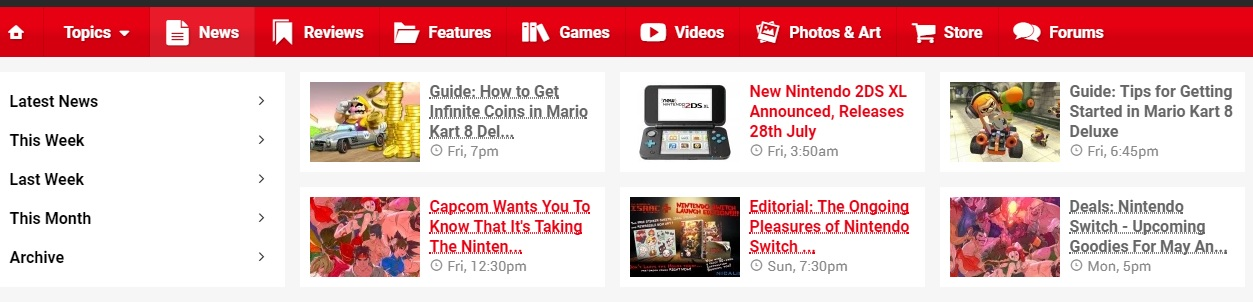
\includegraphics[width=\textwidth]{menu_nav}}
            \caption{\href{pic/menu_nav.jpg}{Menu a comparsa della sezione \emph{news}}\label{fig:menu-nav}}
        \end{figure}
    \end{itemize}
    \item Immediatamente sotto l'header è presente un banner pubblicitario
    \item Subito sotto c'è la \textbf{vetrina} con gli articoli principali del momento, e un altro banner pubblicitario a destra
    \item Sotto comincia la sezione con gli \textbf{articoli} ordinati in ``gruppi'' suddivisi per giorno di pubblicazione. In ogni gruppo gli articoli sono ordinati in modo cronologico secondo la seguente struttura:
    \begin{itemize}
        \item I 2 articoli più recenti sono ingranditi e affiancati.
        \item I successivi 4 articoli sono più piccoli e sono in sequenza verticale, e mostrano anche le prime parole del contenuto.
        \item I restanti sono ancora più piccoli e organizzati in griglia.
    \end{itemize}
    \item A destra della sezione articoli sono presenti vari contenuti consigliati, tra articoli e discussioni sul forum, e collegamenti ai canali social del sito.
    \item Sotto la sezione articoli, è presente una sezione con gli ultimi video pubblicati su \emph{Youtube}, un'altra con le ultime recensioni e, infine, una con le ultime foto postate dai redattori sul canale \emph{Instagram} del sito.
    \item Infine, nel \textbf{footer} e presente una barra di link per la ricerca di titoli che cominciano per una determinata lettera, una griglia contenente link agli articoli più popolari del momento, riferimenti ai profili del sito sui principali social network e link informativi sul sito.
\end{itemize}

\subsubsection{Analisi}
\label{sub:home-analisi}
Come prima impressione, la pagina è sicuramente \textbf{troppo lunga} \xmark: sono richiesti troppi \emph{scroll} per essere vista interamente. Sarebbe stato meglio spezzare il corpo del sito in più pagine (ad esempio, mostrare solo gli articoli e i contenuti di oggi).
Per quanto riguarda i 6 assi informativi, sono state fatte le seguenti osservazioni:
\begin{description}
    \item[Where] (\emph{dove siamo arrivati?}) \hfill \\ Nonostante non sia presente una breve descrizione del sito in cima alla pagina \xmark, è abbastanza chiaro già dal logo e dal nome del sito il contenuto dello stesso \cmark; inoltre, la presenza del pulsante di navigazione \emph{news} relativamente in alto a sinistra nella prima schermata fa intendere che il sito si occupi principalmente di notizie sul mondo Nintendo \cmark.
    \item[Who] (\emph{chi c'è dietro al sito?}) \hfill \\ Non c'è alcuna informazione a riguardo nella prima schermata che l'utente vede \xmark: le uniche informazioni sono presenti nel footer, a più di 10 scroll dall'inizio \xmark.
    \item[Why] (\emph{perché dovrei visitare il sito?}) \hfill \\ Questa domanda viene risposta in maniera implicita dai pulsanti di navigazione dell'header \cmark, che mostrano le varie tipologie di contenuti che il sito offre.
    \item[What] (\emph{che cosa offre il sito?}) \hfill \\  La vetrina è la risposta principale alla domanda \cmark; in misura minore, anche i tasti di navigazione (e i relativi menu a comparsa) mostrano l'offerta del sito \cmark.
    \item[When] (\emph{quali sono le ultime novità del sito?}) \hfill \\ Il pulsante \emph{news} è una delle prime cose che salta all'occhio \cmark; la vetrina riporta gli articoli più recenti e importanti \cmark; infine, la sezione articoli sottostante alla vetrina risponde perfettamente alla domanda \cmark, anche se richiede uno scroll per essere vista \xmark.
    \item[How] (\emph{come arrivo a ciò che mi interessa?}) \hfill \\ La barra di navigazione e i menu a comparsa sono molto efficaci \cmark; inoltre, per gli utenti registrati è possibile usare il menu \emph{hamburger} per arrivare più facilmente ai contenuti per loro interessanti \cmark.
\end{description}
Nel complesso l'utente, a una prima visita, dovrebbe essere in grado di capire facilmente che cosa offre il sito e come usufruirne \cmark.
Altre osservazioni:
\begin{itemize}
    \item[\cmark] Ogni articolo ha un \emph{blurb} che ancicipa brevemente il contenuto dello stesso
    \item[\cmark] Accanto al titolo di ogni articolo, è presente una \emph{keyword} (ben evidenziata) che ne definisce la tipologia (notizia, recensione, anteprima, video, curiosità, \ldots); questo aiuta l'utente a valutare se l'articolo è di suo interesse o meno
    \item[\cmark] L'header e la barra di navigazione compaiono in cima alla finestra se l'utente effettua uno scroll di una pagina verso l'alto; questo accorgimento mitiga il problema dell'eccessiva lunghezza della pagina, evitando all'utente di ritornare all'inizio per usare la barra di navigazione (questo comportamento accade in tutte le pagine del sito)
\end{itemize}